\chapter{开始}
\subsection{开始TensorFlow}
这个向导,你将开始使用TensorFlow编程。在开始本文之前,\href{https://www.tensorflow.org/install/index}{安装TensorFlow}。为了理解这个向导,你将需要:
\begin{itemize}
\item 如何使用Python编程
\item 了解一点数组
\item 了解机器学习更好。即使,你不太了解机器学习,这篇文章仍然应该是你的第一个向导。
\end{itemize}
TensorFlow提供了多个API。最低的TensorFlow 核心API提供给你完整的程序控制。更高级的API构建在TensorFlow核心之上。这些高级API通常比TensorFlow核心更容易阅读和使用。另外,更高级的API使得用户之间重复的任务变得更容易。一像tf.estimator的高级API帮助你管理数据集,estimators,训练和推理。

这个向导以TensorFlow核心开始。之后,我们展示如何在tf.estimators中实现相同的模型。了解TensorFlow核心规则将在你使用更复杂的高级API时给你一个内部工作的思维模型。
\subsection{Tensors}
TensorFlow中数据的核心单元是tensor。一个tensor组成了任意维度数据的值。一个tensor的rank是他的维数。这里有一些例子:
\begin{pythoncode}
# a rank 0 tensor; a scalar with shape []
[1., 2., 3.] # a rank 1 tensor; a vector with shape [3]
[[1., 2., 3.], [4., 5., 6.]] # a rank 2 tensor; a matrix with shape [2, 3]
[[[1., 2., 3.]], [[7., 8., 9.]]] # a rank 3 tensor with shape [2, 1, 3]
\end{pythoncode}
\subsection{TensorFlow核心导航}
\subsubsection{导入TensorFlow}
规范的TensorFlow程序导入如下:
\begin{pythoncode}
import tensorflor as tf 
\end{pythoncode}
这让Python能访问TensorFlow的任何类,方法,符号。多数文档假设你已经有了这。
\subsubsection{计算图}
你也许可以考虑TensorFlow核心程序为下面的两个部分:
\begin{itemize}
\item 构建计算图
\item 运行计算图
\end{itemize}
一个计算图是一系列的安排在图上节点的TensorFlow操作。让我们构建一个简单的计算图,每个节点接收0或者更多的tensor作为输入产生一个tensor作为输出。一个典型的节点是常数。像所有的TensorFlow常数,它不接收输入,输出一个存储在其内部的值。我们可以创建两个浮点Tensor node1和node2:

\begin{pythoncode}
node1 = tf.constant(3.0, dtype=tf.float32)
node2 = tf.constant(4.0) # also tf.float32 implicitly
print(node1, node2)
\end{pythoncode}

最终生成打印:
\begin{pythoncode}
Tensor("Const:0", shape=(), dtype=float32) Tensor("Const_1:0", shape=(), dtype=float32)
\end{pythoncode}
注意打印节点不像你想的那样输出值3.0和4.0,而是他们是节点,当计算时对应的产生3.0和4.0。为了计算节点,你必须用session运行计算图。一个会话是TensorFlow控制和运行环境的集合体。

下面的代码创建一个Session对象,然后调用run方法运行计算图计算node1和node2.默认会话中的计算图如下:
\begin{pythoncode}
sess = tf.Session()
print(sess.run([node1, node2]))
\end{pythoncode}
我们将看到我们想要的输出3.0和4.0:
\begin{pythoncode}
[3.0,4.0]
\end{pythoncode}
你可以通过结合Tensor节点和操作构建更复杂的计算。例如,你可以添加两个常数节点生成一个新的图:
\begin{pythoncode}
from __future__ import print_function
node3 = tf.add(node1, node2)
print("node3:", node3)
print("sess.run(node3):", sess.run(node3))
\end{pythoncode}
最后的打印声明产生:
\begin{pythoncode}
node3: Tensor("Add:0", shape=(), dtype=float32)
sess.run(node3): 7.0
\end{pythoncode}
TensorFlow提供一个称为TensorBoard的实用程序,你可以显示一个计算图。这里的截图显示了TensorBoard如何可视化图:
\begin{figure}[H]
\centering
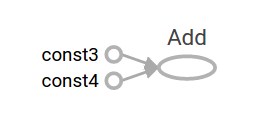
\includegraphics{getting_started_add.png}
\caption{计算图}
\end{figure}
正如上面表示,图并不特别有趣因为它总是产生一个常数结果。一个图可以参数化接收内部输入正如placeholders。一个placeholder
\begin{pythoncode}
a = tf.placeholder(tf.float32)
b = tf.placeholder(tf.float32)
adder_node = a + b  # + provides a shortcut for tf.add(a, b)
\end{pythoncode}
上面的三行代码像一个函数或者lambda表达式,我们定义了两个输入参数(a,b)和一个在他们之上的操作。我们可以通过feed\_dict参数结合多输入计算这个图用\href{https://www.tensorflow.org/api_docs/python/tf/Session#run}{run方法}输入具体的值给placeholders:
\begin{pythoncode}
print(sess.run(adder_node, {a: 3, b: 4.5}))
print(sess.run(adder_node, {a: [1, 3], b: [2, 4]}))
\end{pythoncode}
输出结果:
\begin{pythoncode}
7.5
[ 3.  7.]
\end{pythoncode}
在TensorBoard中图看起来像这样:
\begin{figure}[H]
\centering
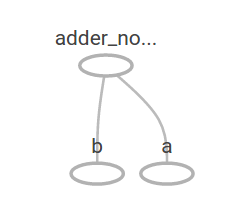
\includegraphics{getting_started_adder.png}
\caption{placeholder}
\end{figure}
你可以通过添加一个另一个操作使得计算图更复杂。例如:
\begin{pythoncode}
add_and_triple = adder_node * 3.
print(sess.run(add_and_triple, {a: 3, b: 4.5}))
\end{pythoncode}
产生输出:22.5。
上面的计算图在TensorBoard中像这样:
\begin{figure}[H]
\centering
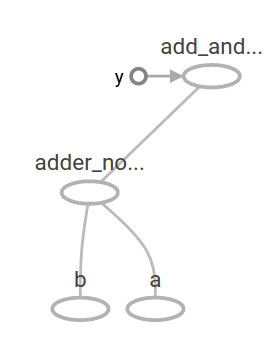
\includegraphics[scale=0.5]{getting_started_triple.png}
\caption{添加操作}
\end{figure}
在机器学习中我们通常接收任意输入,正如上面。为了使得模型可训练,我们需要能修改图获取相同输入的新的输出。Variable允许我们添加可训练的参数到图上。他们通过类型和初始值构造:
\begin{pythoncode}
W = tf.Variable([.3], dtype=tf.float32)
b = tf.Variable([-.3], dtype=tf.float32)
x = tf.placeholder(tf.float32)
linear_model = W*x + b
\end{pythoncode}
当你调用tf.constant时常数被初始化,他们的值不能改改。对比之下,当你调用tf.Variable的时候变量没有被初始化。为了初始化在TensorFlow程序中的所有变量,你必须明确的调用一个像下面的类似操作:
\begin{pythoncode}
init = tf.global_variables_initializer()
sess.run(init)
\end{pythoncode}
实现init处理TensorFlow子图初始化所有变量是很重要的。直到我们调用sess.run,变量才被初始化。
因为x是一个placeholder,我们可以按照下面同时通过多个x计算多个linear\_model:
\begin{pythoncode}
print(sess.run(linear_model, {x: [1, 2, 3, 4]}))
\end{pythoncode}
为了产生输出:
\begin{pythoncode}
[ 0.          0.30000001  0.60000002  0.90000004]
\end{pythoncode}
我们已经创建了一个模型,但是我们不知道它有多么好。为了在训练集上估计模型,我们需要一个placeholder提供想要的值,并且我们需要一个损失函数。

一个损失函数从提供的数据计算模型效果。我们将用标准的线性回归损失函数计算当前模型和提供数据之间的均方差。linear\_model -y创建一个向量,向量的每一个元素是对应的样本的误差。我们可以调用tf.square计算误差的平方,然后我们使用tf.reduce\_sum对所有的误差求和创建一个标量:
\begin{pythoncode}
y = tf.placeholder(tf.float32)
squared_deltas = tf.square(linear_model - y)
loss = tf.reduce_sum(squared_deltas)
print(sess.run(loss, {x: [1, 2, 3, 4], y: [0, -1, -2, -3]}))
\end{pythoncode}
产生损失值23.66。

我们可以通过手动赋值W,h为-1,1做出改变。一个变量被初始化值提供给tf.Variable但是可以使用想tf.assign这样的操作改变。例如,W=-1,和b=1对我们的模型来说是最优的参数。我们可以改变W和b:
\begin{pythoncode}
fixW = tf.assign(W, [-1.])
fixb = tf.assign(b, [1.])
sess.run([fixW, fixb])
print(sess.run(loss, {x: [1, 2, 3, 4], y: [0, -1, -2, -3]}))
\end{pythoncode}
最后的打印结果显示损失现在为0.0。

我们猜测W和b的最佳值,但是机器学习的最终目的是自动找到正确的模型参数。我们将在下面的章节显示如何完成。

\subsubsection{tf.train API}
为了完成这个导航的机器学习讨论。然而,TensorFlow提供优化器通过损失对变量的微分慢慢改变变量的值。通常,手动计算符号微分是很可笑的并且易出错。因此TensorFlow可以使用tf.gradients自动的生成给定描述的模型的微分。简单起见,优化器通常已经为你做好。例如:
\begin{pythoncode}
optimizer = tf.train.GradientDescentOptimizer(0.01)
train = optimizer.minimize(loss)
sess.run(init) # reset values to incorrect defaults.
for i in range(1000):
  sess.run(train, {x: [1, 2, 3, 4], y: [0, -1, -2, -3]})
print(sess.run([W, b]))
\end{pythoncode}
最终模型的参数:
\begin{pythoncode}
[array([-0.9999969], dtype=float32), array([ 0.99999082], dtype=float32)]
\end{pythoncode}
现在我们已经做了实际上的机器学习。尽管这个简单的线性回归模型不要求更多的TensorFlow核心代码,更复杂的输入数据到你的模型的方法需要更多代码。这样TensorFlow提供更高级的的常用样例,结构,功能抽象。我们将在下面的章节学习如何使用这些抽象。
\subsubsection{完整的代码}
完整的训练线性回归模型的代码:
\begin{pythoncode}
import tensorflow as tf

# Model parameters
W = tf.Variable([.3], dtype=tf.float32)
b = tf.Variable([-.3], dtype=tf.float32)
# Model input and output
x = tf.placeholder(tf.float32)
linear_model = W*x + b
y = tf.placeholder(tf.float32)

# loss
loss = tf.reduce_sum(tf.square(linear_model - y)) # sum of the squares
# optimizer
optimizer = tf.train.GradientDescentOptimizer(0.01)
train = optimizer.minimize(loss)

# training data
x_train = [1, 2, 3, 4]
y_train = [0, -1, -2, -3]
# training loop
init = tf.global_variables_initializer()
sess = tf.Session()
sess.run(init) # reset values to wrong
for i in range(1000):
  sess.run(train, {x: x_train, y: y_train})

# evaluate training accuracy
curr_W, curr_b, curr_loss = sess.run([W, b, loss], {x: x_train, y: y_train})
print("W: %s b: %s loss: %s"%(curr_W, curr_b, curr_loss))
\end{pythoncode}
运行产生:
\begin{pythoncode}
W: [-0.9999969] b: [ 0.99999082] loss: 5.69997e-11
\end{pythoncode}
注意损失很小(非常接近于0).如果你运行这个代码,你的损失也许不和上面的损失一样,这是因为模型实用伪随机数值初始化。

更复杂的TensorBoard可视化如下:
\begin{figure}[H]
\centering
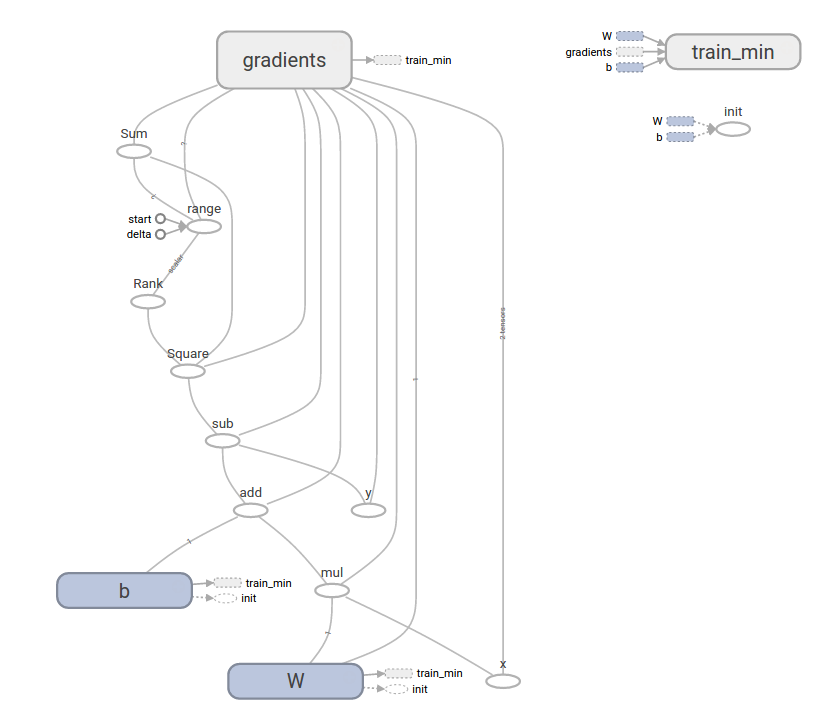
\includegraphics[scale=0.5]{getting_started_final.png}
\caption{整体代码框图}
\end{figure}
\subsubsection{tf.estimators}
tf.estimator是一个改进得TensorFlow库用来简化机器学习机制,包括下面:
\begin{itemize}
\item 运行训练循环
\item 运行估计循环
\item 管理数据集
\end{itemize}
tf.estimators定义了一些常见的模型
\subsubsection{基础用法}
使用tf.estimator线性回归程序变得更简单:
\begin{pythoncode}
# NumPy is often used to load, manipulate and preprocess data.
import numpy as np
import tensorflow as tf

# Declare list of features. We only have one numeric feature. There are many
# other types of columns that are more complicated and useful.
feature_columns = [tf.feature_column.numeric_column("x", shape=[1])]

# An estimator is the front end to invoke training (fitting) and evaluation
# (inference). There are many predefined types like linear regression,
# linear classification, and many neural network classifiers and regressors.
# The following code provides an estimator that does linear regression.
estimator = tf.estimator.LinearRegressor(feature_columns=feature_columns)

# TensorFlow provides many helper methods to read and set up data sets.
# Here we use two data sets: one for training and one for evaluation
# We have to tell the function how many batches
# of data (num_epochs) we want and how big each batch should be.
x_train = np.array([1., 2., 3., 4.])
y_train = np.array([0., -1., -2., -3.])
x_eval = np.array([2., 5., 8., 1.])
y_eval = np.array([-1.01, -4.1, -7, 0.])
input_fn = tf.estimator.inputs.numpy_input_fn(
    {"x": x_train}, y_train, batch_size=4, num_epochs=None, shuffle=True)
train_input_fn = tf.estimator.inputs.numpy_input_fn(
    {"x": x_train}, y_train, batch_size=4, num_epochs=1000, shuffle=False)
eval_input_fn = tf.estimator.inputs.numpy_input_fn(
    {"x": x_eval}, y_eval, batch_size=4, num_epochs=1000, shuffle=False)

# We can invoke 1000 training steps by invoking the  method and passing the
# training data set.
estimator.train(input_fn=input_fn, steps=1000)

# Here we evaluate how well our model did.
train_metrics = estimator.evaluate(input_fn=train_input_fn)
eval_metrics = estimator.evaluate(input_fn=eval_input_fn)
print("train metrics: %r"% train_metrics)
print("eval metrics: %r"% eval_metrics)
\end{pythoncode}
当运行的时候,输出像下面:
\begin{pythoncode}
train metrics: {'average_loss': 1.4833182e-08, 'global_step': 1000, 'loss': 5.9332727e-08}
eval metrics: {'average_loss': 0.0025353201, 'global_step': 1000, 'loss': 0.01014128}
\end{pythoncode}
注意我们的评估数据有一个更高的loss,但是仍然接近于0,这意味了我们正在适当的学习。
\subsubsection{一个自定义的模型}
tf.estimator不限制你使用预先定义的模型。假设我们想创建一个TensorFlow不支持的自定义模型,我们仍然保留数据集的高级抽象,feeding,训练的等等。为了说明这个问题,我们将显示用我们低级API如何实现我们自己的模型LinearRegressor。

为了结合tf.estimator定义自定义的模型,我们需要使用tf.estimator.Estimator。tf.estimator.LinearRegressor实际上是tf.estimator.Estimator的子类。相比于Estimator子类,我们简单提供Estimator一个model\_fn函数高数tf.estimator如何评估预测,训练步数和损失。代码如下:
\begin{pythoncode}
import numpy as np
import tensorflow as tf

# Declare list of features, we only have one real-valued feature
def model_fn(features, labels, mode):
  # Build a linear model and predict values
  W = tf.get_variable("W", [1], dtype=tf.float64)
  b = tf.get_variable("b", [1], dtype=tf.float64)
  y = W*features['x'] + b
  # Loss sub-graph
  loss = tf.reduce_sum(tf.square(y - labels))
  # Training sub-graph
  global_step = tf.train.get_global_step()
  optimizer = tf.train.GradientDescentOptimizer(0.01)
  train = tf.group(optimizer.minimize(loss),
                   tf.assign_add(global_step, 1))
  # EstimatorSpec connects subgraphs we built to the
  # appropriate functionality.
  return tf.estimator.EstimatorSpec(
      mode=mode,
      predictions=y,
      loss=loss,
      train_op=train)

estimator = tf.estimator.Estimator(model_fn=model_fn)
# define our data sets
x_train = np.array([1., 2., 3., 4.])
y_train = np.array([0., -1., -2., -3.])
x_eval = np.array([2., 5., 8., 1.])
y_eval = np.array([-1.01, -4.1, -7., 0.])
input_fn = tf.estimator.inputs.numpy_input_fn(
    {"x": x_train}, y_train, batch_size=4, num_epochs=None, shuffle=True)
train_input_fn = tf.estimator.inputs.numpy_input_fn(
    {"x": x_train}, y_train, batch_size=4, num_epochs=1000, shuffle=False)
eval_input_fn = tf.estimator.inputs.numpy_input_fn(
    {"x": x_eval}, y_eval, batch_size=4, num_epochs=1000, shuffle=False)

# train
estimator.train(input_fn=input_fn, steps=1000)
# Here we evaluate how well our model did.
train_metrics = estimator.evaluate(input_fn=train_input_fn)
eval_metrics = estimator.evaluate(input_fn=eval_input_fn)
print("train metrics: %r"% train_metrics)
print("eval metrics: %r"% eval_metrics)
\end{pythoncode}
当运行时,产生如下:
\begin{pythoncode}
train metrics: {'loss': 1.227995e-11, 'global_step': 1000}
eval metrics: {'loss': 0.01010036, 'global_step': 1000}
\end{pythoncode}
注意自定义的model\_fn()函数的内容类似我们使用低级API训练手动训练模型。

\section{对于ML初学者的MNIST}\label{sec:start}
这个导航针对于对机器学习和TensorFlow生疏的读者。如果你知道MNIST,softmax回归,你最好查看\href{https://www.tensorflow.org/get_started/mnist/pros}{faster paced turotial}。开始任何导航前确保你安装了\href{https://www.tensorflow.org/install/index}{TensorFlow}。
当一个人学习如何编程,他们通常做的第一件事就是打印Hello World。MNIST对于机器学习就像编程的Hello World。

MNIST是一个简单的计算机视觉数据集,由像下面的手写数据组成:
\begin{figure}[H]
\centering
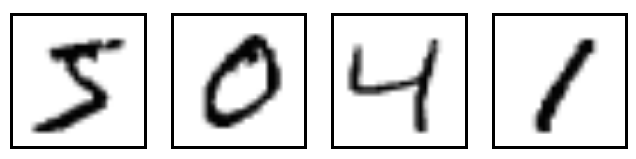
\includegraphics{MNIST.png}
\caption{mnist数据}
\end{figure}
它包含每个图片的标签,高数我们是那个数字。例如,上面的标签分别是5,0,4,1。

在这个导航中,我们将训练一个模型查看图像预测数字。我们的目标不是训练一个真正精巧的模型获取顶尖的性能,尽管我们将在稍后给你代码。但是不是使用TensorFlow简单研究。例如,我们将开始一个非常简单的称为Softmax回归的模型。

实际上代码很短,所有有趣的东西仅仅发生在三行。然而,对于理解它背后的想法却很重要:TensorFlow如何工作和机器学习核心概念。因为这,我们将分厂自己的介绍代码。
\subsection{关于这个导航}
这个导航是一个一行行的解释\href{https://www.github.com/tensorflow/tensorflow/blob/r1.4/tensorflow/examples/tutorials/mnist/mnist_softmax.py}{mnist\_softmax.py}发生了什么。你可以通过两种不同的方法使用这个导航:
\begin{itemize}
\item 当你读每一行解释的时候复制粘贴一行行的每个代码段到Python环境
\item 在你读整个解释致歉运行整个mnist\_softmax.py Python文件,使用导航理解你不清楚的每行代码
在这个导航你将完成:
\item 了解MNIST数据集和softmax回归
\item 创建一个函数模型用于识别,易于图片上的每个像素
\item 通过"看"样本使用TensorFlow训练模型识别数字(运行我们的TensorFlow会话做到)
\item 结合我们的测试数据检查模型的精度
\end{itemize}
\subsection{MNIST数据}
MNIST数据在\href{http://yann.lecun.com/exdb/mnist/}{Yann LeCun's website}。如果你从文档上复制粘贴代码,用下面两行代码开头自动下载读取数据:
\begin{pythoncode}
from tensorflow.examples.tutorials.mnist import input_data
mnist = input_data.read_data_sets("MNIST_data/", one_hot=True)
\end{pythoncode}
MNIST数据分为3部分:55,000训练数据(mnist.train),10,000测试数据(mnist.test)和5,000验证数据(mnist.validation)。这分割很重要:它是机器学习中的基础用来分割数据以至于在没有学习的数据上学到实际上的范化。

正如 我们之前提到的,每个MNIST数据有两部分:手写数字的图片和对应的标签。我们将称为图像"x"和标签"y"。训练集和测试机都包含图像和对应的标签;例如训练图像是mnist.train.images训练标签是mnist.train.labels。

每张图片有$28\times28$像素,我们可以将他解释为一个数组:
\begin{figure}[H]
\centering
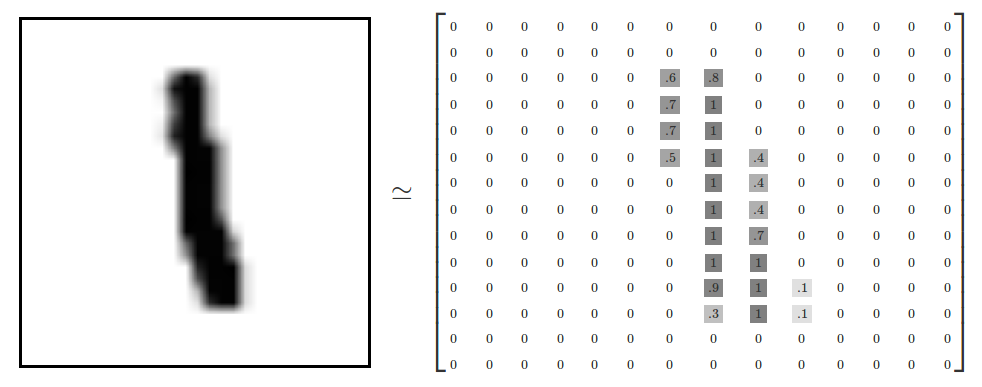
\includegraphics[scale=0.2]{MNIST-Matrix.png}
\caption{图片和对应的矩阵}
\end{figure}
我们可以展开这个数组为一个$28\times28=784$个数的向量。我们如何展开数组不重要只要它和图像一致即可。从这个观点,MNIST图像仅仅是一个\href{https://colah.github.io/posts/2014-10-Visualizing-MNIST/}{very rich structure }784维的向量空间。(警告:计算加强可视化)

展开市局丢掉了图像的2D结构,这很不好?使得最佳的计算机视觉方法利用这个结构,我们将在后面的导航中看到。但是简单的方法softmax回归将在这里使用。

结果时mnist.train.images是一个形状为[55000,784]的tensor(n维)。第一个为都市图像的索引,第二个是索引对应的图像像素。图像中的像素每个tensor的输入是一个0或者1。
\begin{figure}[H]
\centering
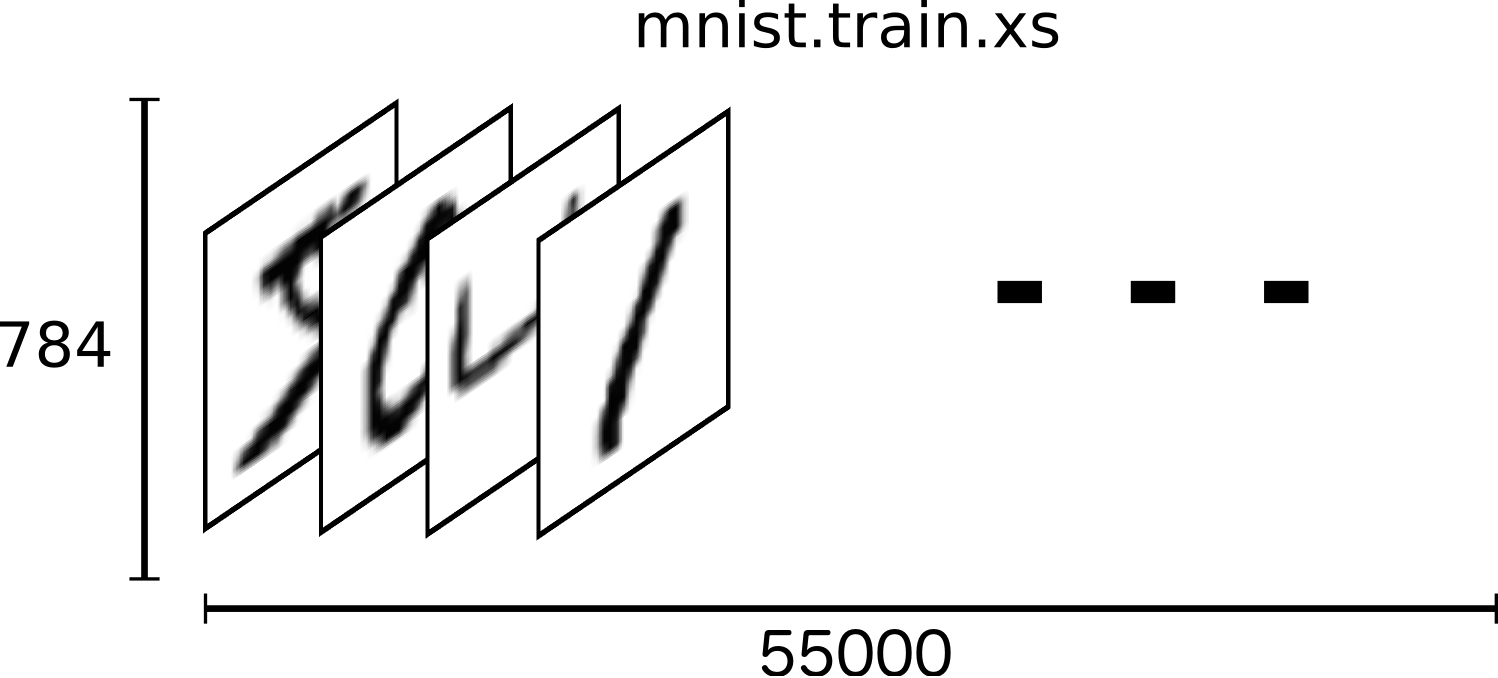
\includegraphics[scale=0.2]{mnist-train-xs.png}
\caption{图像维度}
\end{figure}
每个MNIST中的图像有一个对应的标签,一个0-9的数字,为了达到导航的目的,我们转化我们的标签为“one-hot vector”。一个one-hot向量是一个多数维度上为0,一个维度上1的向量。这种情况下,第n个数字表示维度中第n位置为1.例如3应该是[0,0,0,1,0,0,0,0,0,0]。结果mnist.train.labels是一个[55000,10]的浮点数组。
\begin{figure}[H]
\centering
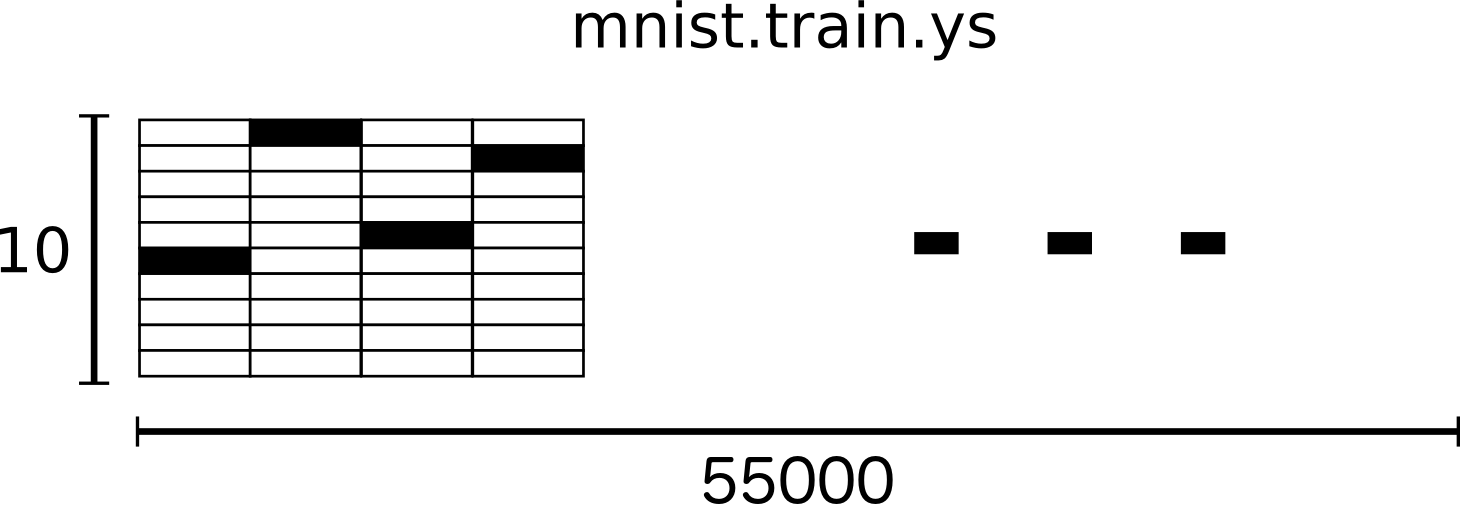
\includegraphics[scale=0.2]{mnist-train-ys.png}
\caption{one-hot vector}
\end{figure}
现在我们准备开始我们的模型。
\subsection{Softmax回归}
我们知道在MNIST中的每张图片是0-9的手写体。因此给定一张图片仅仅只有10个可能。我们想能查看一张图片给定每张图片的概率。例如,我们的模型也许查看图像9 80\%确定是9,5\%确定为8其他的可能性很小因为模型不能100\%确定。

对这个经典的问题softmax恢复是一个自然,简单的模型。如果你想复制概率给一个对象成为多个不同对象中的一个,softmax做的就是这个,因为softmax给0-1的输出。在之后当我们训练更加精妙的模型,最后的步骤将是一个softmax操作。

一个softmax回归有两部:首先我们添加在确定类别中的输入,然后我们转化输出概率。为了总结一个类别的概率,如果它被支持我们权衡像素强度。

下面的图显示了从这些类别权衡一个模型。红色表示负权重,蓝色表示正权重。

\begin{figure}[H]
\centering
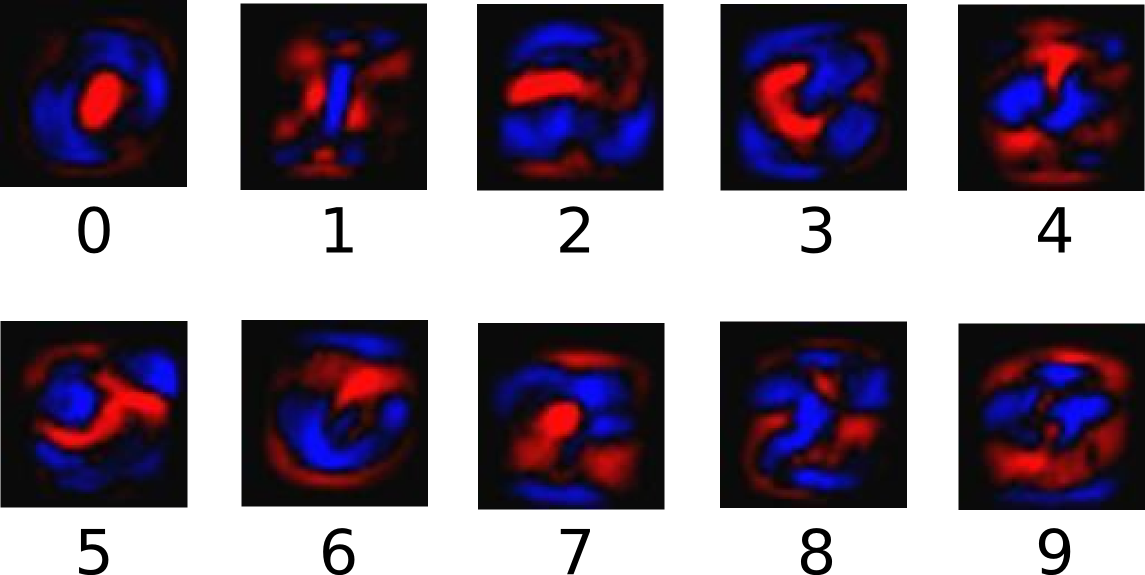
\includegraphics[scale=0.2]{softmax-weights.png}
\caption{softmax手写体}
\end{figure}
我们添加额外的偏执。基本上,我们想能说一些事更可能和输入独立。结果时给定输入x了类别i结果是:
\[evidence_i = \sum_{j}W_{i,j}x_j+b_i\]
这里的$W_i$是权重$b_i$是类别i偏置,j是在我们的输入图像x上的求和的索引。我们使用softmax转化evidence为我们的预测概率y:
\[y=softmax(evidence)\]
这里的softmax作为一个激活函数或者链接函数,输出我们线性函数为我们想要的。在这种情况下,概率分布在10个类别上。我们可以认为转化依据为我们输入每个类别的概率,定义如下:
\[softmax(evidence)=normalize(exp(evidence))\]
如果你展开方程,你得到:
\[softmax(evidence)_i = \frac{exp(evidence_i)}{\sum_jexp(evidence_j)}\]
但是首先考虑softmax方法京城很有用:指数输入和归一化。指数平均一个单元增加权重到任何假设。相反有更少的证据意味着假设获取之前前中的一部分。没哟偶假设有0或者负权重。fostmax然后归一化权重,以至于相加为1。形成一个可用的概率分布。(为了说明softmax函数,查看Michael Nielsen的数的\href{http://neuralnetworksanddeeplearning.com/chap3.html#softmax}{章节},完全的交互式可视化。)

你可以想下面画softmax回归,尽管有更多的x。对于每个输入,我们计算x的加权和加上偏执使用softmax。
\begin{figure}[H]
\centering
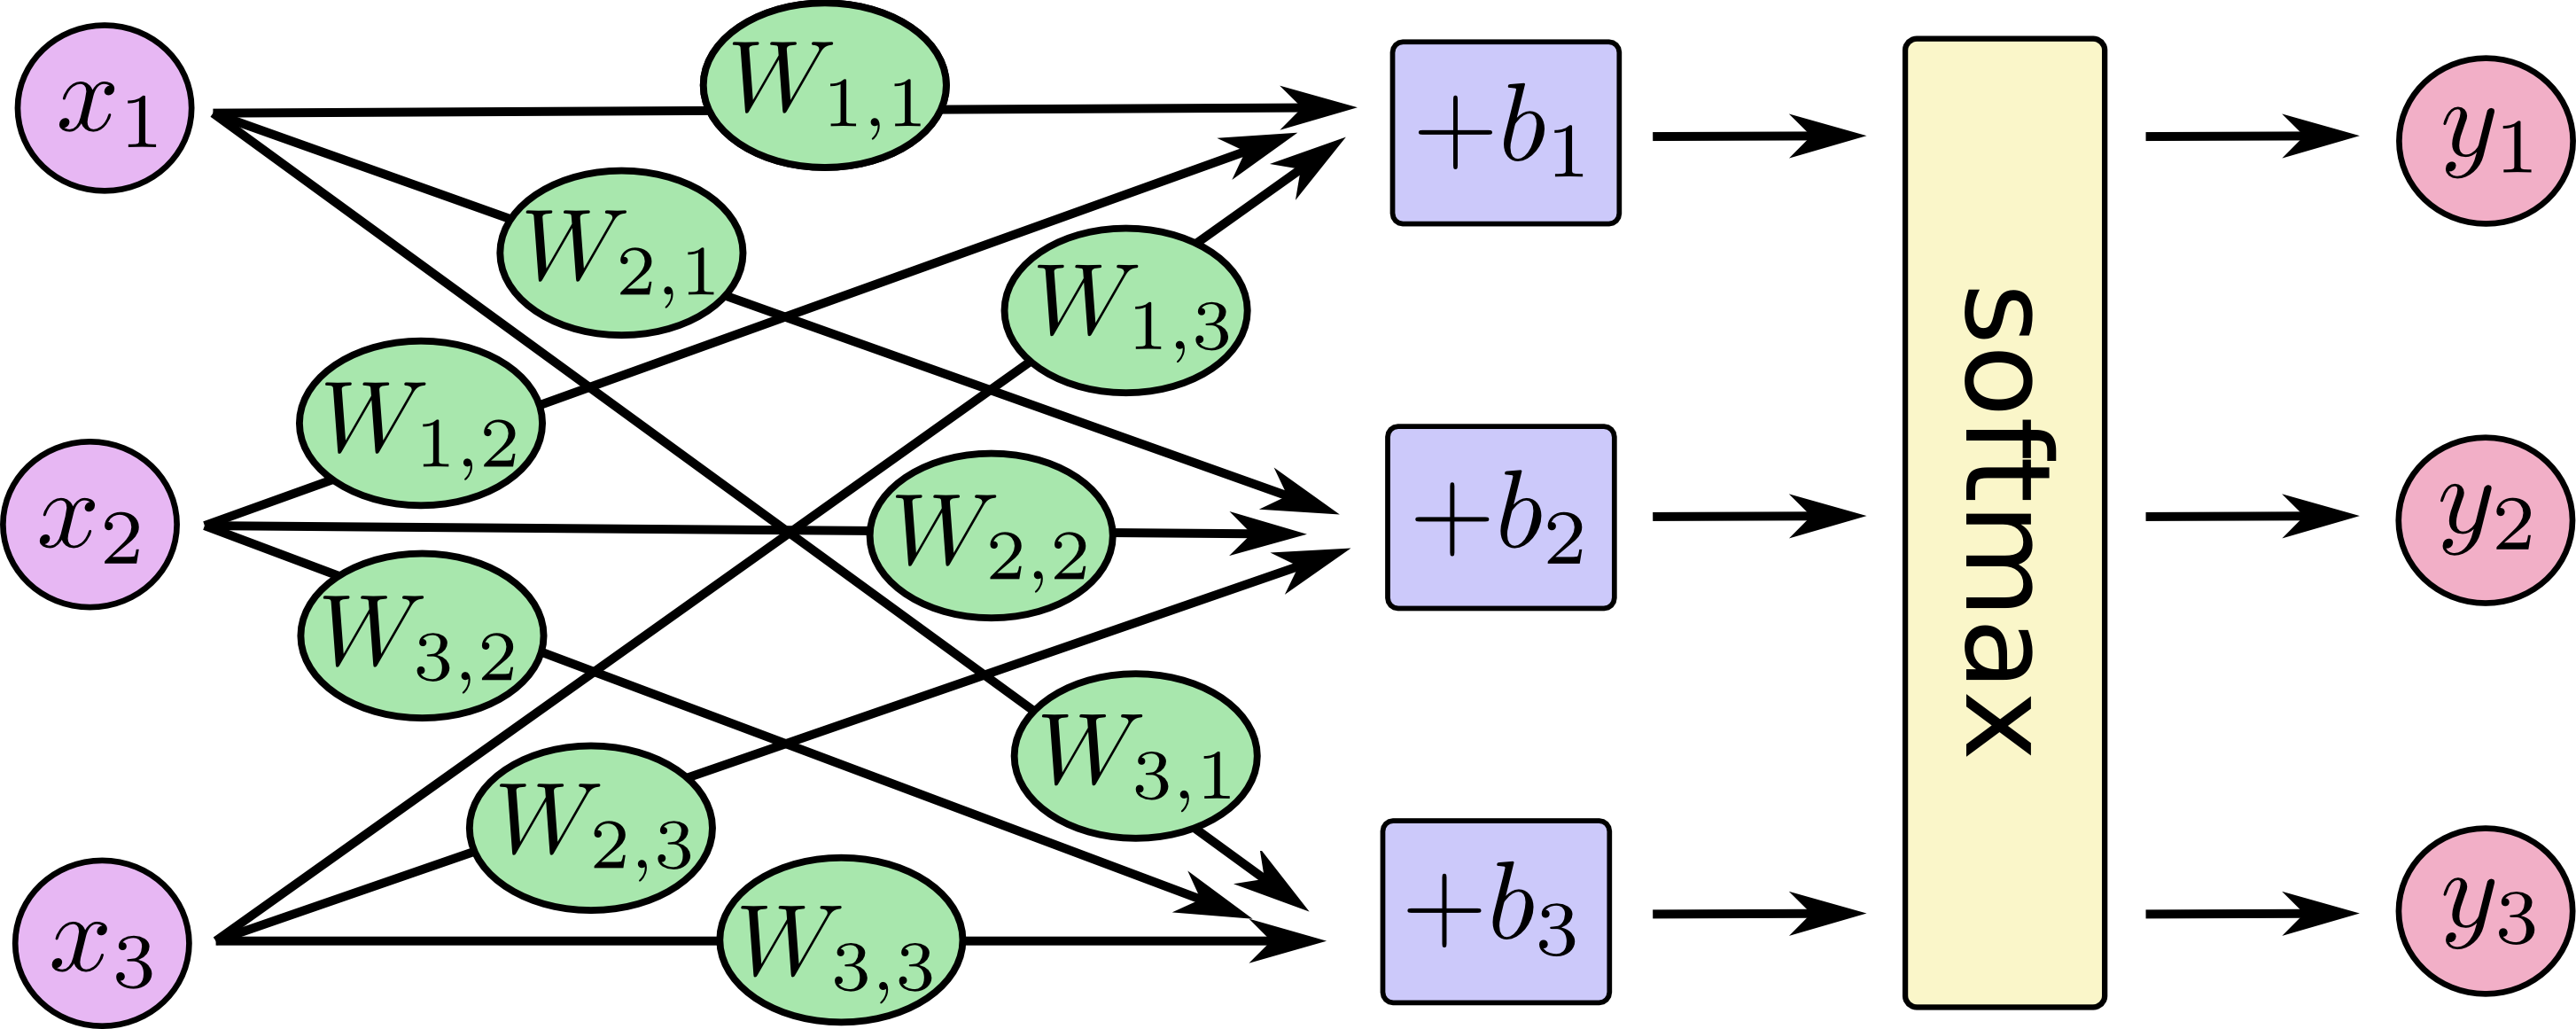
\includegraphics[scale=0.1]{softmax-regression-scalargraph.png}
\caption{softmax计算过程}
\end{figure}
如果你写为方程,你得到:
\begin{figure}[H]
\centering
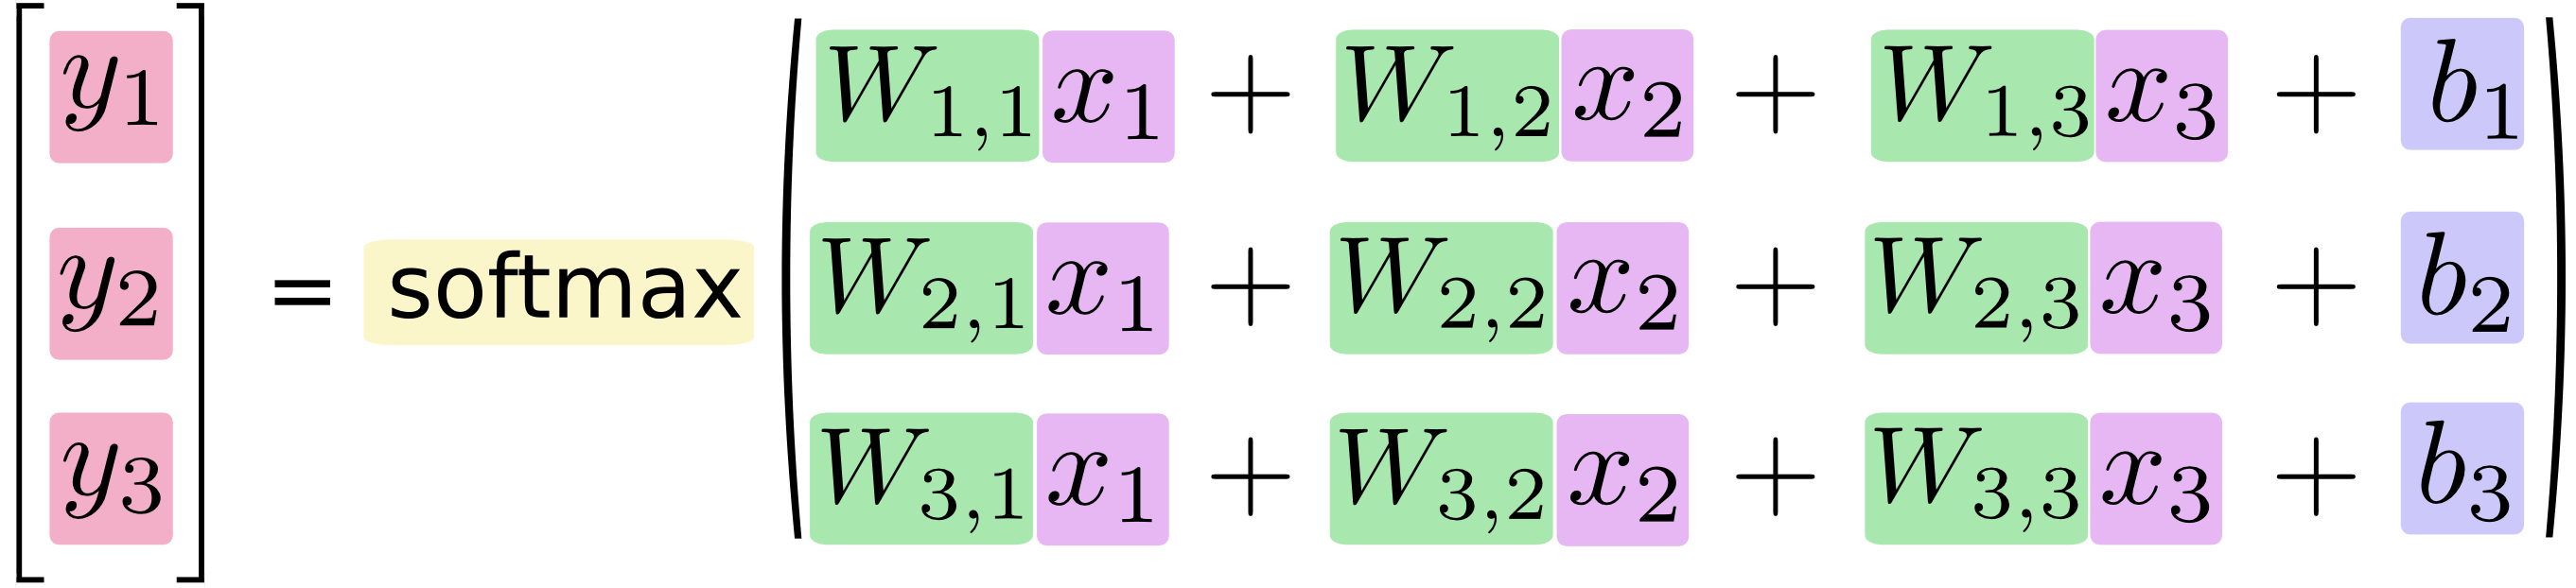
\includegraphics[scale=0.1]{softmax-regression-scalarequation.png}
\caption{softmax 方程}
\end{figure}
我们可以向量化这个过程,转变他为一个矩阵惩罚和向量加。这对于高效计算很有用(它总是一个有用的思考方法)。
\begin{figure}[H]
\centering
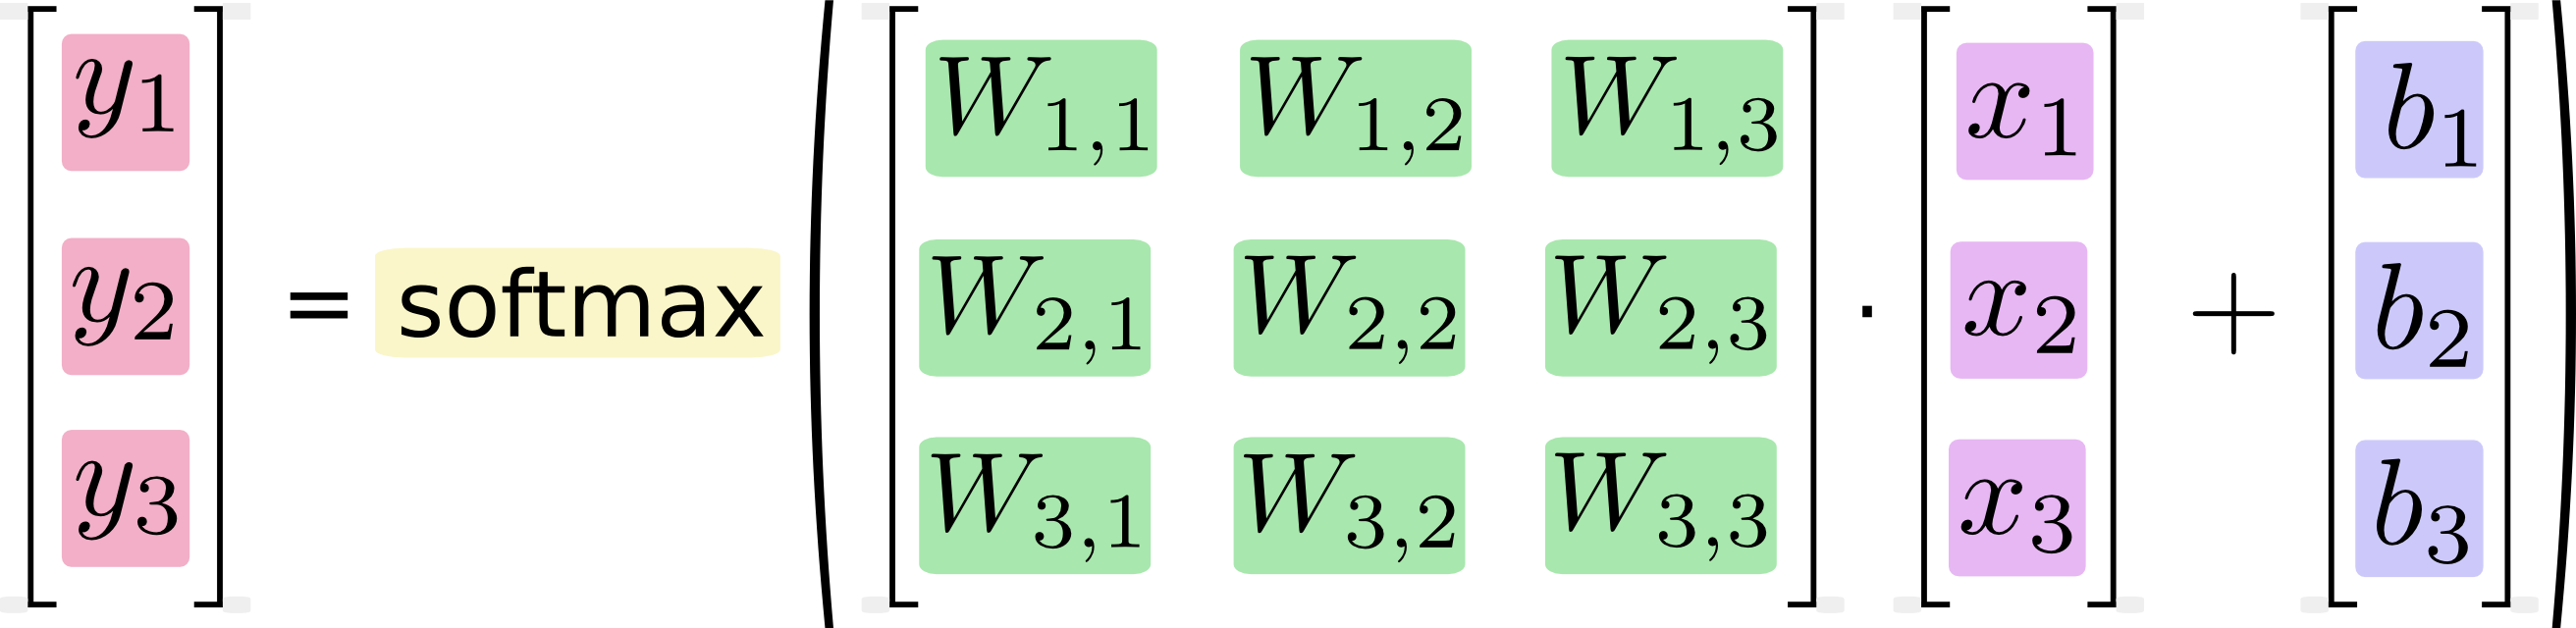
\includegraphics[scale=0.1]{softmax-regression-vectorequation.png}
\caption{向量化的softmax}
\end{figure}
更加简洁的你可以这样写:
\[y=fostmax(Wx+b)\]
现在我们使用TensorFlow转化它。
\subsection{实现回归}
为了在Python中进行的数值计算,我们通常使用一个\href{http://www.numpy.org/}{NumPy}库在Python外使用其他其他语言的高效实现做代价高昂的矩阵乘法操作。不幸的是转化每个操作会Python的时候依然有一些开销。如果你在GPU或者是分布式环境(这里我们转化数据代价很高)中使用是开销特别大。

TensorFlow也在Python外做了提升,但是对于减小开销减少有一点作用。想不语从Python运行的代价,TensorFlow让我们在Python外描述交互的操作。(这样的方法可以在一些机器学习库中看到)

为了使用TensorFlow,首先导入他。
\begin{ipythoncode}
import tensorflow as tf 
\end{ipythoncode}
我们通过符号变量描述交互的操作,让我们创建一个:
\begin{ipythoncode}
x = tf.placeholder(tf.float32, [None, 784])
\end{ipythoncode}
x没有指定值。是一个当我们要求TensorFlow运行时放置值的placholder。我们想能输入任意数量的MNIST图像,每张图像展开为784维(这里的None意味着这一维度可以为任意长度)
我们也需要权重和偏执用于计算。我们可以想象这些为额外的输入,但是TensorFlow有更好的处理方法:Variable。一个Variable是在TensorFlow图上的交互操作的一个可修改的tensor。他可以通过计算使用和修改。对于机器学习应用,一个常规的模型参数为Variable。
\begin{pythoncode}
W = tf.Variable(tf.zeros([784, 10]))
b = tf.Variable(tf.zeros([10]))
\end{pythoncode}
我们通过tf.Variable创建这些Variable初始化variable的值:在这种情况下,我们初始化W和b作为全0 tensor。因此我们将学习W和b。他们初始化为什么不重要。注意W形状为[784,10]因为我们想乘784维图像向量生成10维不同类别可信向量。b形状为[10]因此可以添加到输出。我们可以用一行定义实现我们的模型:
\begin{pythoncode}
y = tf.nn.softmax(tf.matmul(x, W) + b)
\end{pythoncode}
首先我们用tf.matmul(x,w)乘上x和W。它可我们方程用颠倒了这里是$Wx$作为结合多输入一个处理x为2D tensor的技巧。我们然后添加b最后使用tf.nn.softmax

这里我们使用了一行定义我们的模型,之后的一些行设置。这是不是因为TensorFlow设计就是为了做一个特别容易的regression:它仅仅是一个灵活的描述一些种类数值计算的方法,通过机器学习模型护理方针。一旦定义,我们的模型可以再不同的设备上运行:你的电脑的CPU,GPU甚至手机!

\subsubsection{训练}
为了定义我们的模型,我们需要定义什么方法对我们的模型来说很好。实际上机器学习中我们通常定义它意味着模型将变差。我们调用这个cost或者loss表达我们的模型和我们想要的输出之间的差距。我们尝试最小化误差,误差越小,模型越好。

通常,很简单的决定模型损失的函数为交叉熵(cross-entropy),交叉熵在信息论中提出考虑信息压缩编码,但是在一些淋雨,想机器学习领域变成了一个重要的想法,如下定义
\[H_y'(y)=-\sum_iy_i'log(y_i)\]
这里的y是我们的预测的概率分布,$y'$是真是的分布(数字的One-hot向量)。简单说交叉熵是衡量我们的预测对于真实的描述有多搞笑。详细的交叉熵介绍超过了这个导航范围,但是值得\href{https://colah.github.io/posts/2015-09-Visual-Information}{理解}。

为了实现交叉熵我们需要添加一个新的placeholder到输入正确的回答:
\begin{pythoncode}
y_ = tf.placeholder(tf.float32, [None, 10])
\end{pythoncode}
然后我们可以实现交叉熵函数$-\sum y'log(y)$:
\begin{pythoncode}
cross_entropy = tf.reduce_mean(-tf.reduce_sum(y_ * tf.log(y), reduction_indices=[1]))
\end{pythoncode}
首先,tf.log计算每个元素y的对数。下一步,我们乘上每个输入$y\_$和对应的tf.log(y)。然后tf.reduce\_sum添加元素在y的第二维,由于reduction\_indices=[1]参数。最后,tf.redce\_mean计算所有在batch中的样本的均值。

注意在源代码中,我们没有使用这个公式,因为这是数值不稳定的。取而代之的是我们shiyongtf.nn.softmax\_cross\_entropy\_with\_ligits在为最这话的logits(例如我们调用softmax\_cross\_entropy\_with\_logits在tf.matmul(x,W)+b)上,因为在更数值稳定函数内部计算softmax激活。在你的代码中,考虑使用tf.nn.softmax\_cross\_entropy\_with\_logits代替。
现在我们知道我们想让我们的模型做什么,对TensorFlow训练来说很容易。因为TensorFlow知道我们的整个计算图,这可以通过\href{https://colah.github.io/posts/2015-08-Backprop}{反向传播}搞笑的决定你的变量如何影响你想最小化的loss。这可以使用你的优化算法又该边疆减少loss。
\begin{pythoncode}
train_step = tf.train.GradientDescentOptimizer(0.5).minimize(cross_entropy)
\end{pythoncode}
在这种强狂下,我们要求TensorFlow通过学习率0.5的\href{https://en.wikipedia.org/wiki/Gradient_descent}{梯度下降算法}最小化交叉熵。梯度下降算法是一个简单的处理,这里TensorFlow简单的在cost见效的方向转变每个变量一点点。但是TensorFlow也提供\href{https://www.tensorflow.org/api_guides/python/train#Optimizers}{一些其他的优化算法}和上面一样简单的一行。

TensorFlow在这里做了什么,背后的机制是添加新的操作到图上实现反向传播和梯度下降。然后它给你返回一个操作,当运行的时候,体恤下降训练,轻微的转变你的变量减少损失。

我们可以在InteractiveSession启动模型:
\begin{pythoncode}
sess = tf.InteractiveSession()
\end{pythoncode}
我们首先必须创建一个操作初始化我们创建的变量:
\begin{pythoncode}
tf.global_variables_initializer().run()
\end{pythoncode}
让我们训练,我们将训练100次!
\begin{pythoncode}
for _ in range(1000):
  batch_xs, batch_ys = mnist.train.next_batch(100)
	  sess.run(train_step, feed_dict={x: batch_xs, y_: batch_ys})
\end{pythoncode}
循环的每一步,我们从我们的训练集上得到100个batch随机的数据点。我们运行train\_step输入批数据代替placeholder。

使用晓得batch随机数据成为随机训练,在这种情况下。最佳的我们想在每部使用所有的我们的数据因为浙江给我们一个更好的关于我们应该做什么的理解。但是这代价带。因此,作为替代,我们每次用一个不同的子集。作者有相同的好处代价更低。
\subsubsection{评估我们的模型}
我们的模型效果怎样?
首先让我们找出预测争取的标签。tfargmax是一个极其有用的函数给你沿着一个轴最高的输入tensor的索引。例如,tf.argmax(y,1)是我们的模型对于输入的认为最可能的标签,然而tf.ragmax(y\_1,1)是正确的标签。我们可以使用tf.equal检查是否我们的预测和真实情况匹配。
\begin{pythoncode}
correct_prediction = tf.equal(tf.argmax(y,1), tf.argmax(y_,1))
\end{pythoncode}
这给我们一个boolean列表。为了决定什么部分是正确的,我们转化为浮点数然后平均。例如[True,False,True,True]将被转化为[1,0,1,1]为0.75。
\begin{pythoncode}
accuracy = tf.reduce_mean(tf.cast(correct_prediction, tf.float32))
\end{pythoncode}
最后我们获取我们的测试集上的精度:大约92\%
\begin{pythoncode}
print(sess.run(accuracy, feed_dict={x: mnist.test.images, y_: mnist.test.labels}))
\end{pythoncode}
这很好?不,事实上,很差。这是因为我们使用了一个非常简单的模型。结合一些改变,我们可以得到97\%。最好的模型可以达到99.7\%的精度(更多信息查看\href{https://rodrigob.github.io/are_we_there_yet/build/classification_datasets_results}{结果列表})

我们从这个模型学到的重要的。一球,如果你正对结果感到沮丧。查看\href{https://www.tensorflow.org/get_started/mnist/pros}{下一个导航}这里我们使用TensorFlow做了一些更好的,学习构建更多精妙的模型。
\section{针对专家的深度MNIST}
TensorFlow是一个强大的大规模数值计算库。这里一个任务是实现和训练深度神经网络。在这个导航我们将学习基本的构造TensorFlow模块构造深度卷积MNIST分类器。

这个介绍假设你熟悉想MNIST数据集和神经网络。如果你没有相关背景查看\ref{sec:start}。开始导航前确保TensorFlow被安装了。

\subsection{关于这个导航}
这个导航的第一部分解释在\href{https://www.github.com/tensorflow/tensorflow/blob/r1.4/tensorflow/examples/tutorials/mnist/mnist_softmax.py}{mnist\_softmax.py}代码,一个基础的TensorFlow模型。第二部分显示提高精度的一些方法。
你可以从这个导航复制粘贴相关代码段到Python环境,或者你可以下载完整的代码实现\href{https://www.github.com/tensorflow/tensorflow/blob/r1.4/tensorflow/examples/tutorials/mnist/mnist_softmax.py}{mnist\_softmax.py}

我们将在这个导航中完成:
\begin{itemize}
\item 基于看到的每一个像素为识别MNIST数字创建一个softmax回归函数
\item 使用TensorFlow训练模型通过"看"很多样本识别数字(运行我们的第一个TensorFlow会话)
\item 使用我们的测试集检查模型的精度
\item 构建,训练测试多层卷积神经网络改进结果
\end{itemize}
\subsection{开始}
在开始创建我们的模型前,我们将首先载入MNIST数据集开始TensorFlow会话。
\subsection{载入MNIST数据集}
如果你从这个导航复制粘贴代码,以这两行开始将自动的下载读入数据:
\begin{pythoncode}
from tensorflow.examples.tutorials.mnist import input_data
mnist = input_data.read_data_sets('MNIST_data', one_hot=True)
\end{pythoncode}
这里的mnist是一个轻量级的存储numpy数组训练,验证,测试集。它也踢动一个函数通过minibatch迭代。
\subsection{开始TensorFlow交互式会话(InteractiveSession)}
TensorFlow依赖于一个搞笑的C++后端计算。连接到后端成为一个会话。通常使用TensorFlow程序首先创建一个图然后在会话中启动它。

这里我们使用方便的交互式会话类,使得TensorFlow能更灵活的构造你的代码。它允许你交互操作构建一个\href{https://www.tensorflow.org/get_started/get_started#the_computational_graph}{计算图}然后运行图。这当你在想IPython这样的交互式环境中使用是很方便。如果你没有使用一个交互式会话,然后在你开启一个会话前你应该构建整个计算图启动图。
\begin{pythoncode}
import tensorflow as tf
sess = tf.InteractiveSession()
\end{pythoncode}
\subsection{计算图}
为了在Python中搞笑的处理数值计算,我们通过使用一个想\href{http://www.numpy.org/}{Numpy}的库在Python外通过其它语言实现的高效代码做代价高昂的矩阵乘法。不幸的是转换回Python每个操作任然有一些开销。如果你在分布式环境或者在GPU上计算这些开销将很巨大,这里转换数据代价很高。

TensorFlow在Python外做计算量重的工作,但是进一步避免这开销。从Python外运行带个的昂贵的操作,TensorFlow让我们描述操作交互的图然后子啊Python外运行。这方法类似于Theano和Torch。

Python代码的角色是构建这个外部计算图,然后指示计算图的那一部分应该运行。查看\ref{sec:start}计算图章节获取更多细节。
\section{构造Softmax回归模型}
在这个章节我们将使用单层线性层构建一个softmax回归模型。在下一个章节,我们将结合多层卷及网络扩展这个层到softmax回归。
\subsection{Placeholders}
我们通过为输入图像和输出目标创建节点构建计算图。
\begin{pythoncode}
x = tf.placeholder(tf.float32, shape=[None, 784])
y_ = tf.placeholder(tf.float32, shape=[None, 10])
\end{pythoncode}
这里的x和y\_没有指定值。而是他们都是值在TensorFlow运行计算图时才需要值的placeholder。输入图像x包含2维浮点数tensor。这里指定shape是[None,784],这里的784是$28\times28$像素的MNIST图像,None表示第一个维度,表示输入的批的大小,可以使任意大小。目标输出类别y\_由2dtensor组成。这里每一行对应一个one-hot编码的向量(9个0一个1).shape参数对于placeholder是可选的,但是它允许TensorFlow自动从已经构造的tensor捕获形状。
\subsection{变量}
我们现在为我们的模型定义权重W和偏置b。我们可以将他们当做额外的输入,但是TensorFlow有更好的方法处理他们。Variable是一个TensorFlow计算图中的值。他可以在计算中使用甚至修改。在机器学习应用中,一个常用的模型蚕食是Variable。
\begin{pythoncode}
W = tf.Variable(tf.zeros([784,10]))
b = tf.Variable(tf.zeros([10]))
\end{pythoncode}
我们调用tf.Variable为每个参数传递初始值。在这里我们初始化W和b为全领,W是一个$784\times10$的矩阵(应为我们有784输入和10个特征),b是一个10维的向量(因为有10个类别)。在Variable被session使用之前,他们必须被初始化。这一步接受初始值(这个例子中全0)已经指定,指定他们到每个Variable。可以通过:
\pythoninline{sess.run(tf.global_variables_initializer())}

\subsection{预测类别和损失函数}
我们现在实现了我们的回归模型。它仅仅一行!我们乘上向量化的输入图像x和权重矩阵W,添加偏执。
\pythoninline{y = tf.matmul(x,W)+b}

为了简单的指定一个损失函数。损失函数预示着模型的预测在单一样本上的好坏;我们尝试在所有的样本中最小化它。这里我们的损失韩式是目标个softmax激活函数应用到模型预测上的交叉熵。正如导航的开始,我们用稳定的公式:
\begin{pythoncode}
cross_entropy = tf.reduce_mean(
    tf.nn.softmax_cross_entropy_with_logits(labels=y_, logits=y))
\end{pythoncode}
注意tf.nn.softmax\_cross\_entropy\_with\_digits内部使用softmax在模型的未正则画的模型预测和求和所有的类,tf.reduce\_mean在这些求和上求平均。
\subsection{训练模型}
现在我们已经定义了我们的模型和训练损失函数,直接使用TensorFlow训练。因为TensorFlow知道整个计算图,他可以自动微分找到损失对于每个变量的梯度。TensorFlow有一些\href{https://www.tensorflow.org/api_guides/python/train#optimizers}{內建优化算法}。例如我们使用steepest梯度下降,设置步长为0.5下降交叉熵。
\pythoninline{train_step = tf.train.GradientDescentOptimizer(0.5).minimize(cross_entropy)}

在这一行代码中我们实际上添加一个新的操作到计算图上。操作包含计算梯度,每步更新参数,应用更新参数。

返回的操作train\_step然后运行,将应用梯度下降算法更新参数。训练模型因此可以被通过运行train\_step结合
\begin{pythoncode}
for _ in range(1000):
  batch = mnist.train.next_batch(100)
  train_step.run(feed_dict={x: batch[0], y_: batch[1]})
\end{pythoncode}
我们每次迭代训练时载入100训练样本。我们然后运行train\_step操作,使用feed\_dict取代placeholder tensor想和y\_。注意你可以使用feed\_dict替换在你的计算图中的任何tensor,而不仅仅是placeholder。
\subsection{评估模型}
我们的模型效果怎么样?

首先我们找出我们模型预测正确的标签。tf.argmax是一个极其有用的函数用来给你沿着某一轴最大值的索引。例如,tf.argmax(y,1)是每个我们模型认为的每个输出的标签,然而tf.argmax(y\_,1)是真实标签。我们可以使用tf.equal检查还是否我们的预测和真实值相同。\newline
\pythoninline{correct_prediction = tf.equal(tf.argmax(y,1), tf.argmax(y_,1))}

这将给我们一个bool列表。为了变成分数,我们转化点浮点数然后求平均。例如[True,False,True,True]将编程[1,0,1,1]为0.75。\newline
\pythoninline{accuracy = tf.reduce_mean(tf.cast(correct_prediction, tf.float32))}
最后我们计算我们在测试数据上的精度。应该大约为92\%
\pythoninline{print(accuracy.eval(feed_dict={x: mnist.test.images, y_: mnist.test.labels}))}

\section{构建多层卷积网络}

在MNIST上获得了大约92\%的精确度是很差的。在这章我们将修复它,从单个模型到现代高级模型:一个晓得卷积网络。浙江让我们获得大约99.2\%的精度。

这里的图使用TensorBoard创建:
\begin{figure}[H]
\centering
\includegraphics[scale=0.5]{mnist_deep.png}
\caption{深度MNIST}
\end{figure}
\subsection{权重初始化}
为了创建这个模型,我们将需要创建一些权重。通常初始化权重的时候给一点噪声打破对称性以阻止0梯度。因此我们使用\href{https://en.wikipedia.org/wiki/Rectifier_(neural_networks)}{ReLU}神经元,它用晓得正初始化偏执初始化他们避免"死神经元"。为了避免重复做这个工作我们构建模型,让我们手动创建两个函数:
\begin{pythoncode}
def weight_variable(shape):
  initial = tf.truncated_normal(shape, stddev=0.1)
  return tf.Variable(initial)

def bias_variable(shape):
  initial = tf.constant(0.1, shape=shape)
  return tf.Variable(initial)
\end{pythoncode}
\subsection{卷积和池化}
TensorFlow给我们一些灵活的卷积和池化操作。如何处理边界?stride大小多少?在这个例子中,我们选择vanilla版本。我们的卷积使用zero padding因此输出和输入形状相同。我们的池化是一个普通的$2\times2$最大池化。为了使得代码更清晰,我们抽象这些操作为函数。
\begin{pythoncode}
def conv2d(x, W):
  return tf.nn.conv2d(x, W, strides=[1, 1, 1, 1], padding='SAME')

def max_pool_2x2(x):
  return tf.nn.max_pool(x, ksize=[1, 2, 2, 1],
                        strides=[1, 2, 2, 1], padding='SAME')
\end{pythoncode}
\subsection{第一个卷基层}
我们现在实现我们的第一层。他将由卷积最大池化组成。卷积将为$5\times5$path计算32特征。他的权重的形状为[5,5,1,32],前两维是patch的大小,第三个为输入的通道,最后一维是输出的通道,我们将有一个输出通道组层的偏置向量
\begin{pythoncode}
W_conv1 = weight_variable([5, 5, 1, 32])
b_conv1 = bias_variable([32])
\end{pythoncode}
为了应用这层,我们首先reshapex为一个4维tensor,第二第三维度对应图像的宽度和高度,最后一维对应颜色通道数。\newline
\pythoninline{x_image = tf.reshape(x, [-1, 28, 28, 1])}
我们然后卷积x\_image和权重tensor,添加偏置,应用ReLU函数,最后最大池化。max\_pool\_2x2方法将减少图像的尺寸为$14\times14$
\begin{pythoncode}
h_conv1 = tf.nn.relu(conv2d(x_image, W_conv1) + b_conv1)
h_pool1 = max_pool_2x2(h_conv1)
\end{pythoncode}
\subsection{第二层卷积}
为了构建一个深度网络,我们堆叠一些这种类型的层。第二层有64个$5\times5$特征的特征。
\begin{pythoncode}
W_conv2 = weight_variable([5, 5, 32, 64])
b_conv2 = bias_variable([64])

h_conv2 = tf.nn.relu(conv2d(h_pool1, W_conv2) + b_conv2)
h_pool2 = max_pool_2x2(h_conv2)
\end{pythoncode}
\subsection{Densely连接层}
现在图像的大小已经减小到$7\times7$,我们添加全连接的层到1024个神经元允许处理整张图片。我们reshape池化层的tensor到一批向量,乘上权重矩阵,添加偏执,应用ReLU。
\begin{pythoncode}
W_fc1 = weight_variable([7 * 7 * 64, 1024])
b_fc1 = bias_variable([1024])

h_pool2_flat = tf.reshape(h_pool2, [-1, 7*7*64])
h_fc1 = tf.nn.relu(tf.matmul(h_pool2_flat, W_fc1) + b_fc1)
\end{pythoncode}
\subsection{Dropout}
为了减少过拟合,我们应用输出层\href{https://www.cs.toronto.edu/~hinton/absps/JMLRdropout.pdf}{dropout}。我们创建一个placeholder保存神经元输出的比率。这允许我们在训练中转化dropout,在测试是关闭。TensorFlow的tf.nn.dropout添加mask在神经元上操作自动处理缩放神经元输出,因此dropout仅仅没有任何额外缩放的时候有效。
\begin{pythoncode}
keep_prob = tf.placeholder(tf.float32)
h_fc1_drop = tf.nn.dropout(h_fc1, keep_prob)
\end{pythoncode}
\subsection{输出层}
最后我们添加一个层,就好像在上面应用softmax回归一样
\begin{pythoncode}
W_fc2 = weight_variable([1024, 10])
b_fc2 = bias_variable([10])

y_conv = tf.matmul(h_fc1_drop, W_fc2) + b_fc2
\end{pythoncode}
\subsection{训练和评估模型}
我们的模型怎么样?为了训练和评估它,我们将使用和单层softmax网络几乎一样的代码。不同在一:
\begin{itemize}
\item 我们将替换steepest梯度下降优化器为更加陷阱的ADAM优化器
\item 我们将包含额外的参数keep\_prob到feed\_dict控制drpout率
\item 我们将在每次训练进程中每100次迭代采集一次
\end{itemize}
我们将使用tf.Session而不是tf.InteractiveSession。更好的区分创建图(模型指定)和评估图(模型拟合)。通常使得代码更清晰。tf.Session通过
\href{https://docs.python.org/3/whatsnew/2.6.html#pep-343-the-with-statement}{with block}创建因此在块退出后将自动销毁。
运行这代码,考虑做20000次训练迭代休息一会(可能话半小时),取决于你的处理器速度。
\begin{pythoncode}
cross_entropy = tf.reduce_mean(
    tf.nn.softmax_cross_entropy_with_logits(labels=y_, logits=y_conv))
train_step = tf.train.AdamOptimizer(1e-4).minimize(cross_entropy)
correct_prediction = tf.equal(tf.argmax(y_conv, 1), tf.argmax(y_, 1))
accuracy = tf.reduce_mean(tf.cast(correct_prediction, tf.float32))

with tf.Session() as sess:
  sess.run(tf.global_variables_initializer())
  for i in range(20000):
    batch = mnist.train.next_batch(50)
    if i % 100 == 0:
      train_accuracy = accuracy.eval(feed_dict={
          x: batch[0], y_: batch[1], keep_prob: 1.0})
      print('step %d, training accuracy %g' % (i, train_accuracy))
    train_step.run(feed_dict={x: batch[0], y_: batch[1], keep_prob: 0.5})

  print('test accuracy %g' % accuracy.eval(feed_dict={
      x: mnist.test.images, y_: mnist.test.labels, keep_prob: 1.0}))
\end{pythoncode}
最后的测试机精度应该近似99.2\%。
我们已经学习了如何使用TensorFlow快速简单的构建,训练,评估高级深度学习模型。
